\subsection{構築技術}

構築技術は、実際にコードや実行可能なソフトウェアを作るための具体的な方法である。この章では、API、オブジェクト指向、総称、表明、例外処理、実行可能モデル、状態機械、設定、国際化、構文解析、並行処理、ミドルウェア、分散・クラウド、異種システム、性能、標準、テストファースト、フィードバックループを扱う。

\subsubsection{API の設計と利用}

API は、ライブラリやフレームワーク、サービスを利用するために公開された操作の集合である。API は、関数名や引数の型といった署名だけでなく、その操作が何を意味し、どのような効果を持つかという意味も含む。

よい API は、学びやすく、覚えやすく、読みやすいコードにつながり、誤用しにくく、拡張しやすく、必要な機能を十分に備え、後方互換性を保ちやすい。広く使われるライブラリやサービスでは、実装よりも API の方が長く生きることが多いため、API は安定性が重要である。

Web API では、RESTful API や OpenAPI のような標準的な記述がよく使われる。API ファーストとは、アプリケーションの内部実装より先に API の契約を設計し、その契約に基づいてサーバ側とクライアント側を作る考え方である。

\par\smallskip
\begin{center}
\centering
\IfFileExists{assets/generated_figures/ch04/fig-ch04-08.png}{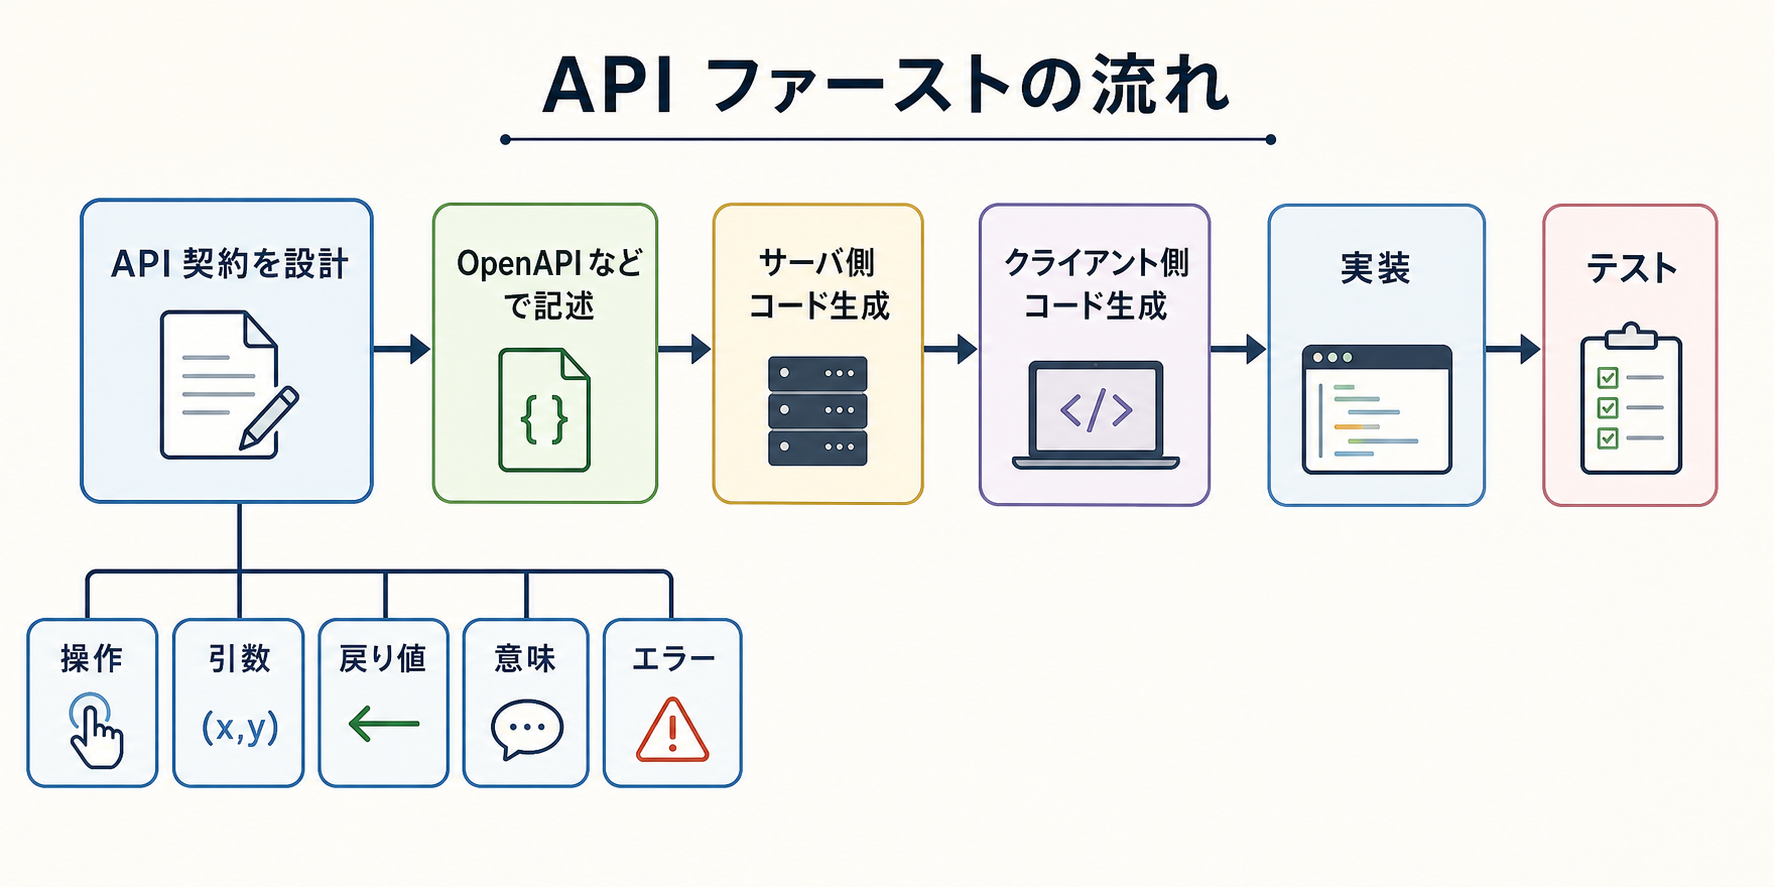
\includegraphics[width=0.96\linewidth]{assets/generated_figures/ch04/fig-ch04-08.png}}{\fbox{\parbox[c][48mm][c]{0.9\linewidth}{\centering 画像生成待ち\\API ファーストの流れ}}}
\par\smallskip
\refstepcounter{figure}\label{fig:ch04-08}図 \thefigure: API ファーストの流れ
\end{center}
図 \thefigure は、API ファーストの流れを視覚的に整理したものである。
\par\smallskip

\subsubsection{オブジェクト指向の実行時問題}

オブジェクト指向言語には、実行時に振る舞いを決める仕組みがある。代表例は多態性と反射である。

多態性とは、一般的な操作を、実際の具体的なオブジェクトの種類に応じて実行時に決められる性質である。たとえば、同じ「描画する」という操作でも、円、四角形、文字列で実行される処理が異なる。このように実行時に呼び出し先が決まることを動的束縛という。

反射とは、プログラムが実行時に自分自身の構造や振る舞いを調べたり、変更したりできる性質である。たとえば、クラス名やメソッド名を文字列として扱い、実行時にオブジェクトを生成したり、メソッドを呼び出したりできる。

これらは柔軟性を高めるが、理解やテストを難しくすることがある。利用する場合は、意図を明確にし、過度に動的な構造を避ける必要がある。

\subsubsection{パラメータ化、テンプレート、総称}

パラメータ化された型は、型やクラスを定義するときに、利用する型の一部を後から与えられるようにする仕組みである。Java では総称、C++ ではテンプレートと呼ばれる。

たとえば、整数のリスト、文字列のリスト、顧客オブジェクトのリストを別々に作るのではなく、「任意の型 T のリスト」として定義し、利用時に T を指定できる。これにより、型安全性を保ちながら再利用しやすい部品を作れる。

\subsubsection{表明、契約による設計、防御的プログラミング}

表明とは、プログラム中に置かれる実行可能な条件式である。プログラムが想定する前提や不変条件が成り立っているかを実行時に確認する。開発時には欠陥を早く見つける助けになる。

契約による設計とは、各関数やクラスについて、呼び出し前に満たすべき事前条件、呼び出し後に保証する事後条件、常に守られる不変条件を明確にする考え方である。これにより、部品同士の責任範囲が明確になる。

防御的プログラミングとは、不正な入力や想定外の状態から関数を守るために、入力値を検査し、異常な場合の処理を決めることである。防御的に書くことで、欠陥の影響を局所化しやすい。

\par\smallskip
\begin{center}
\centering
\IfFileExists{assets/generated_figures/ch04/fig-ch04-09.png}{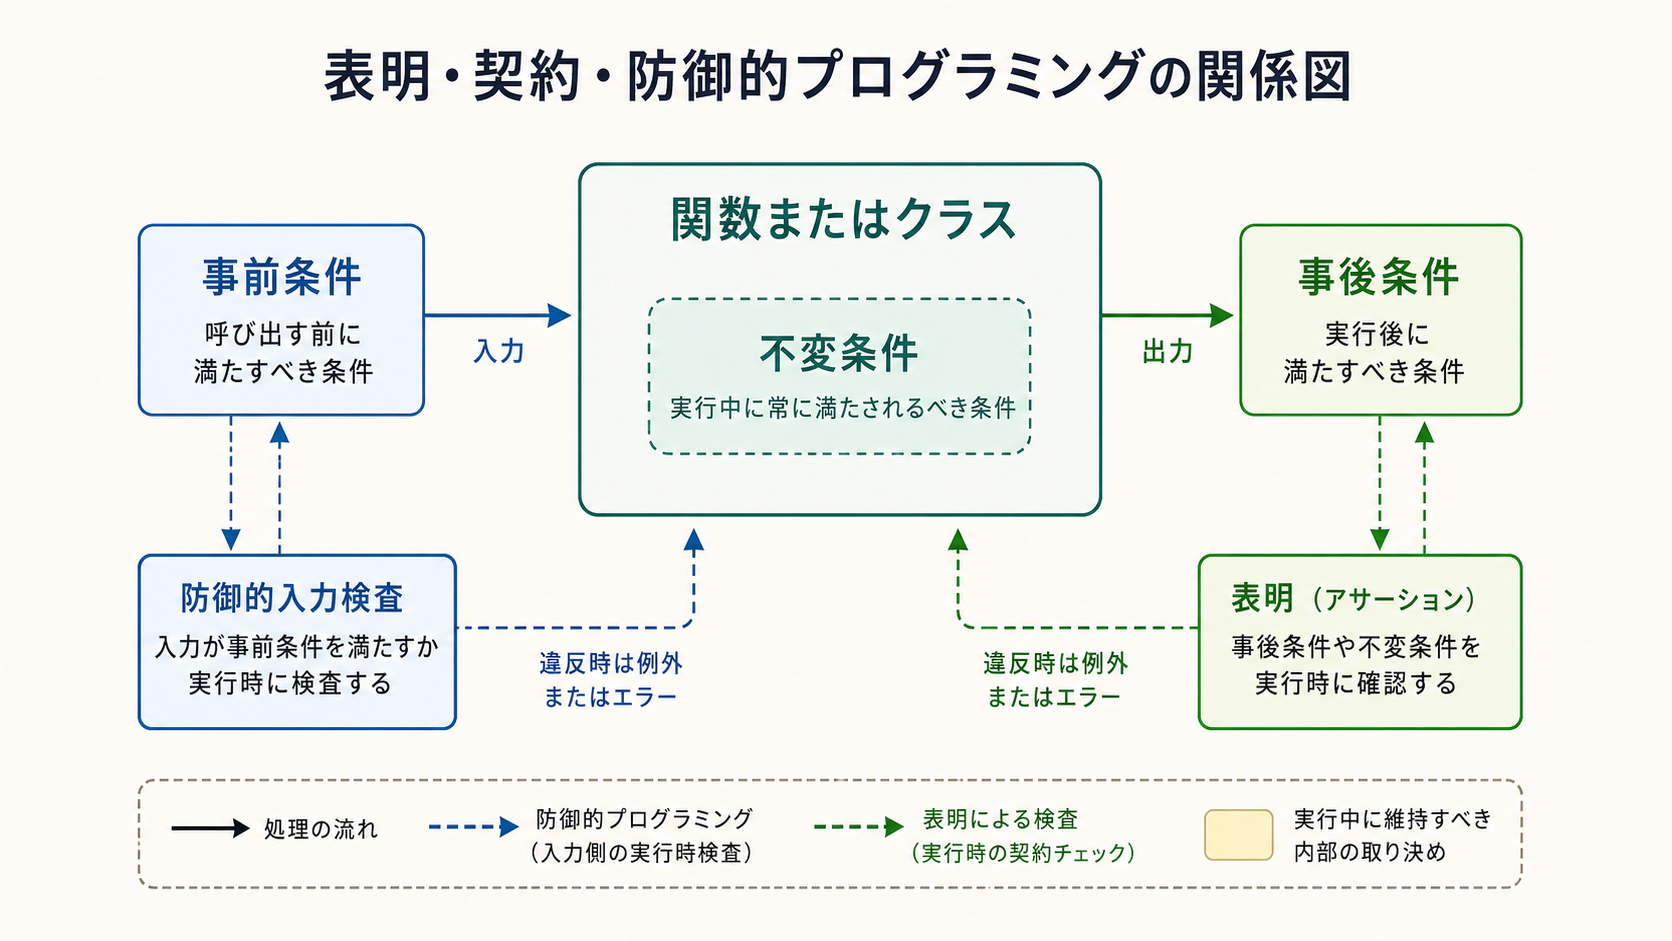
\includegraphics[width=0.96\linewidth]{assets/generated_figures/ch04/fig-ch04-09.png}}{\fbox{\parbox[c][48mm][c]{0.9\linewidth}{\centering 画像生成待ち\\表明・契約・防御的プログラミングの関係図}}}
\par\smallskip
\refstepcounter{figure}\label{fig:ch04-09}図 \thefigure: 表明・契約・防御的プログラミングの関係図
\end{center}
図 \thefigure は、表明・契約・防御的プログラミングの関係図を視覚的に整理したものである。
\par\smallskip

\subsubsection{エラー処理、例外処理、フォールトトレランス}

エラー処理の方法は、正しさ、頑健性、信頼性に影響する。エラー処理には、警告ログを出す、エラーコードを返す、中立値を返す、次の有効データを使う、処理を停止するなど、複数の方法がある。どれを使うかは、利用者への影響、データの重要性、安全性、復旧可能性によって変わる。

例外処理は、エラーや例外的な出来事を検出し、処理する仕組みである。基本的には、例外を送出し、対応する処理ブロックで捕捉する。例外メッセージには、原因理解に必要な情報を含めるべきである。空の捕捉ブロックで例外を握りつぶすと、問題の発見が遅れる。

フォールトトレランスとは、エラーを検出し、回復するか、影響を閉じ込めることで、ソフトウェアの信頼性を高める技法群である。再試行、補助コード、投票アルゴリズム、値の代替などがある。

\subsubsection{実行可能モデル}

実行可能モデルとは、特定のプログラミング言語や実装構造の詳細から離れて、実行できる形で振る舞いを表すモデルである。実行可能 UML などが例である。

モデル駆動アーキテクチャでは、プラットフォーム非依存モデルとプラットフォーム固有モデルを区別する。プラットフォーム非依存モデルは、実装環境に依存しない解決策を表す。プラットフォーム固有モデルは、特定のハードウェアやソフトウェア環境の詳細を含む。変換器は、非依存モデルとプラットフォーム情報を組み合わせ、実装を生成する。

\par\smallskip
\begin{center}
\centering
\IfFileExists{assets/generated_figures/ch04/fig-ch04-10.png}{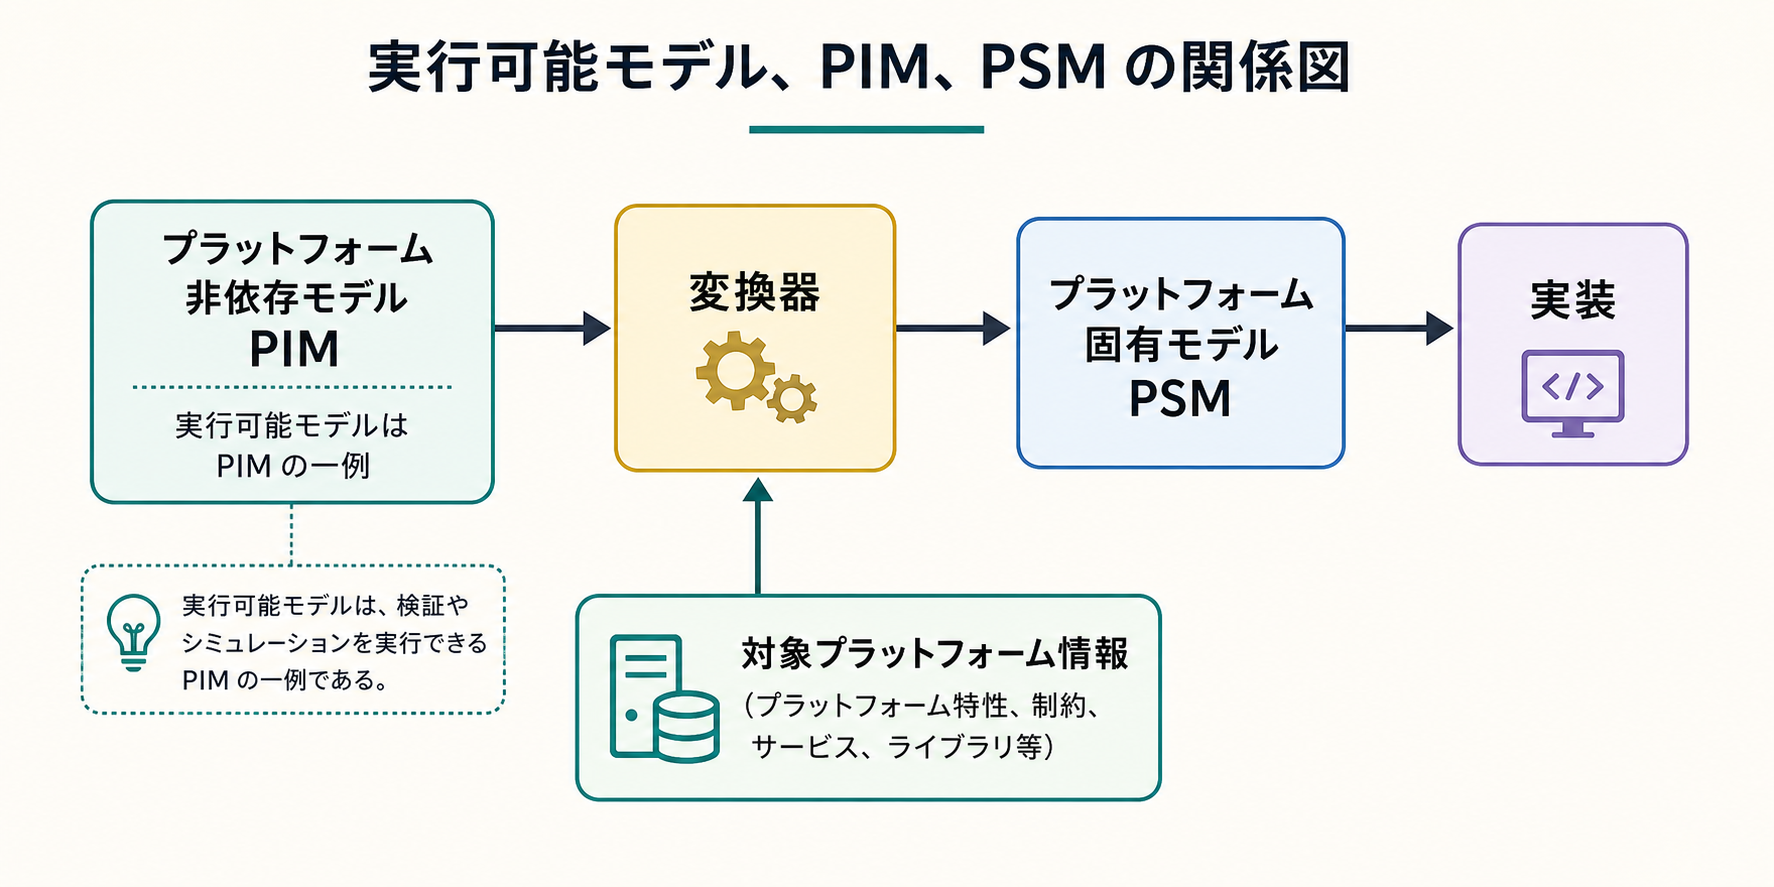
\includegraphics[width=0.96\linewidth]{assets/generated_figures/ch04/fig-ch04-10.png}}{\fbox{\parbox[c][48mm][c]{0.9\linewidth}{\centering 画像生成待ち\\実行可能モデル、PIM、PSM の関係図}}}
\par\smallskip
\refstepcounter{figure}\label{fig:ch04-10}図 \thefigure: 実行可能モデル、PIM、PSM の関係図
\end{center}
図 \thefigure は、実行可能モデル、PIM、PSM の関係図を視覚的に整理したものである。
\par\smallskip

\subsubsection{状態に基づく構築技法と表駆動構築技法}

状態に基づくプログラミングは、有限状態機械を使ってプログラムの振る舞いを表す技法である。状態、イベント、遷移、動作を明確にすることで、複雑な分岐を整理できる。状態遷移図は、仕様、実装、デバッグ、文書化で使える。

表駆動方式は、複雑な \texttt{if} 文や \texttt{case} 文の代わりに、表を使って情報を表す方法である。条件と処理の対応を表にまとめると、ロジックが見通しやすく、変更もしやすくなることがある。表駆動では、何を表に入れるか、どのように効率よく表を参照するかが重要である。

\par\smallskip
\begin{center}
\centering
\IfFileExists{assets/generated_figures/ch04/fig-ch04-11.png}{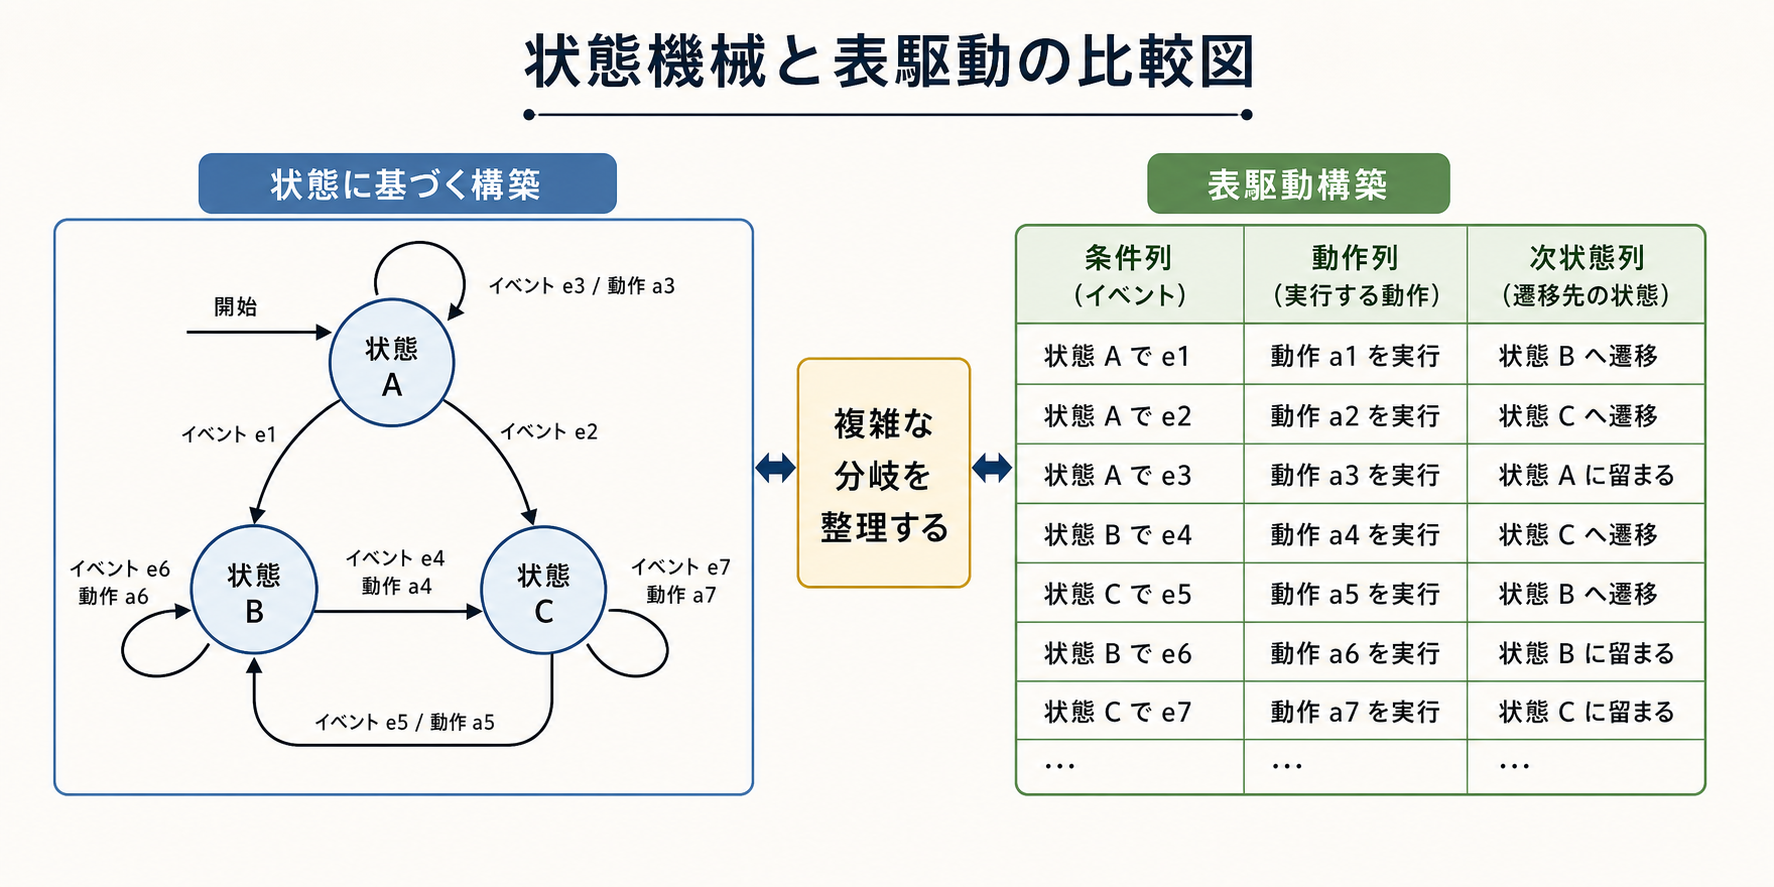
\includegraphics[width=0.96\linewidth]{assets/generated_figures/ch04/fig-ch04-11.png}}{\fbox{\parbox[c][48mm][c]{0.9\linewidth}{\centering 画像生成待ち\\状態機械と表駆動の比較図}}}
\par\smallskip
\refstepcounter{figure}\label{fig:ch04-11}図 \thefigure: 状態機械と表駆動の比較図
\end{center}
図 \thefigure は、状態機械と表駆動の比較図を視覚的に整理したものである。
\par\smallskip

\subsubsection{実行時設定と国際化}

実行時設定とは、プログラムの値や動作を、実行時に設定ファイルや環境変数などから読み取って決めることである。これにより、コードを変更せずに動作を変えられる。設定を使うことで柔軟性は高まるが、設定値の検証、既定値、変更履歴、機密情報の扱いが重要になる。

国際化とは、複数の言語や地域に対応できるようにソフトウェアを準備することである。これに対応して、特定の地域や言語に合わせる作業を地域化という。画面の文言、エラーメッセージ、日付形式、通貨、文字コード、並び順、右から左へ書く言語などを考慮する必要がある。

国際化を後から追加すると、コードのあちこちに埋め込まれた文字列や地域依存の処理を修正する必要がある。構築時から、文字列を外部化し、文字コードとロケールを意識することが重要である。

\subsubsection{文法に基づく入力処理}

\term{文法}{Grammar}に基づく入力処理は、入力を字句や構文の規則に従って解析する技法である。代表的な例は、プログラミング言語、設定ファイル、数式、検索式、通信プロトコルの解析である。

構文解析では、入力のトークン列から解析木または構文木と呼ばれるデータ構造を作る。解析木は、その入力がどのような構造を持つかを表す。構文解析の後、意味検査やシンボル表の確認を行い、計算処理や変換処理につなげる。

文法に基づく入力処理は、入力検証にも重要である。曖昧な文字列処理で入力を解釈すると、誤解析やセキュリティ問題につながる可能性がある。

\subsubsection{並行処理の基本部品}

並行処理では、複数の処理が同時または並行して進む。共有資源に同時にアクセスすると競合が起こるため、同期の仕組みが必要である。代表的な基本部品には、セマフォ、モニタ、ミューテックスがある。

セマフォは、複数のプロセスやスレッドが共有資源へアクセスする数を制御するための抽象である。モニタは、共有変数とその操作をひとまとまりにし、同時に一つの処理だけが内部で動くようにする抽象データ型である。ミューテックスは、共有資源への排他的アクセスを実現するための仕組みである。

並行処理の欠陥は再現しにくいことが多い。デッドロック、競合状態、ライブロック、可視性の問題などを避けるには、設計段階から同期方針を明確にし、テストとレビューを組み合わせる必要がある。

\subsubsection{ミドルウェア}

ミドルウェアとは、オペレーティングシステムより上、アプリケーションより下で、アプリケーションに共通サービスを提供するソフトウェアである。通信、メッセージング、永続化、トランザクション、名前解決、位置透過性などを提供することがある。

ミドルウェアは、部品同士を接続する役割を持つ。メッセージ指向ミドルウェアは、複数のアプリケーション間のメッセージ交換を支援する。企業サービスバスは、サービス指向の通信や連携を支える基盤として使われる。

\subsubsection{分散およびクラウド基盤ソフトウェアの構築方法}

分散システムは、物理的に離れた複数の計算機がネットワークで接続され、利用者に一体の資源や機能を提供するシステムである。分散ソフトウェアの構築では、並列性、通信、遅延、部分故障、整合性、セキュリティが問題になる。

分散プログラミングには、クライアントサーバ、三層アーキテクチャ、多層アーキテクチャ、分散オブジェクト、疎結合、密結合などの形がある。

クラウド基盤ソフトウェアでは、マイクロサービス、コンテナ、API ゲートウェイ、サービス登録と発見、監視、自動スケーリングなどを考慮する。従来の分散トランザクションでは ACID 特性を重視することが多い。一方、マイクロサービスでは、すべてを強い整合性で統一するのが難しく、SAGA などによる結果整合性を使うことがある。

\par\smallskip
\begin{center}
\centering
\IfFileExists{assets/generated_figures/ch04/fig-ch04-12.png}{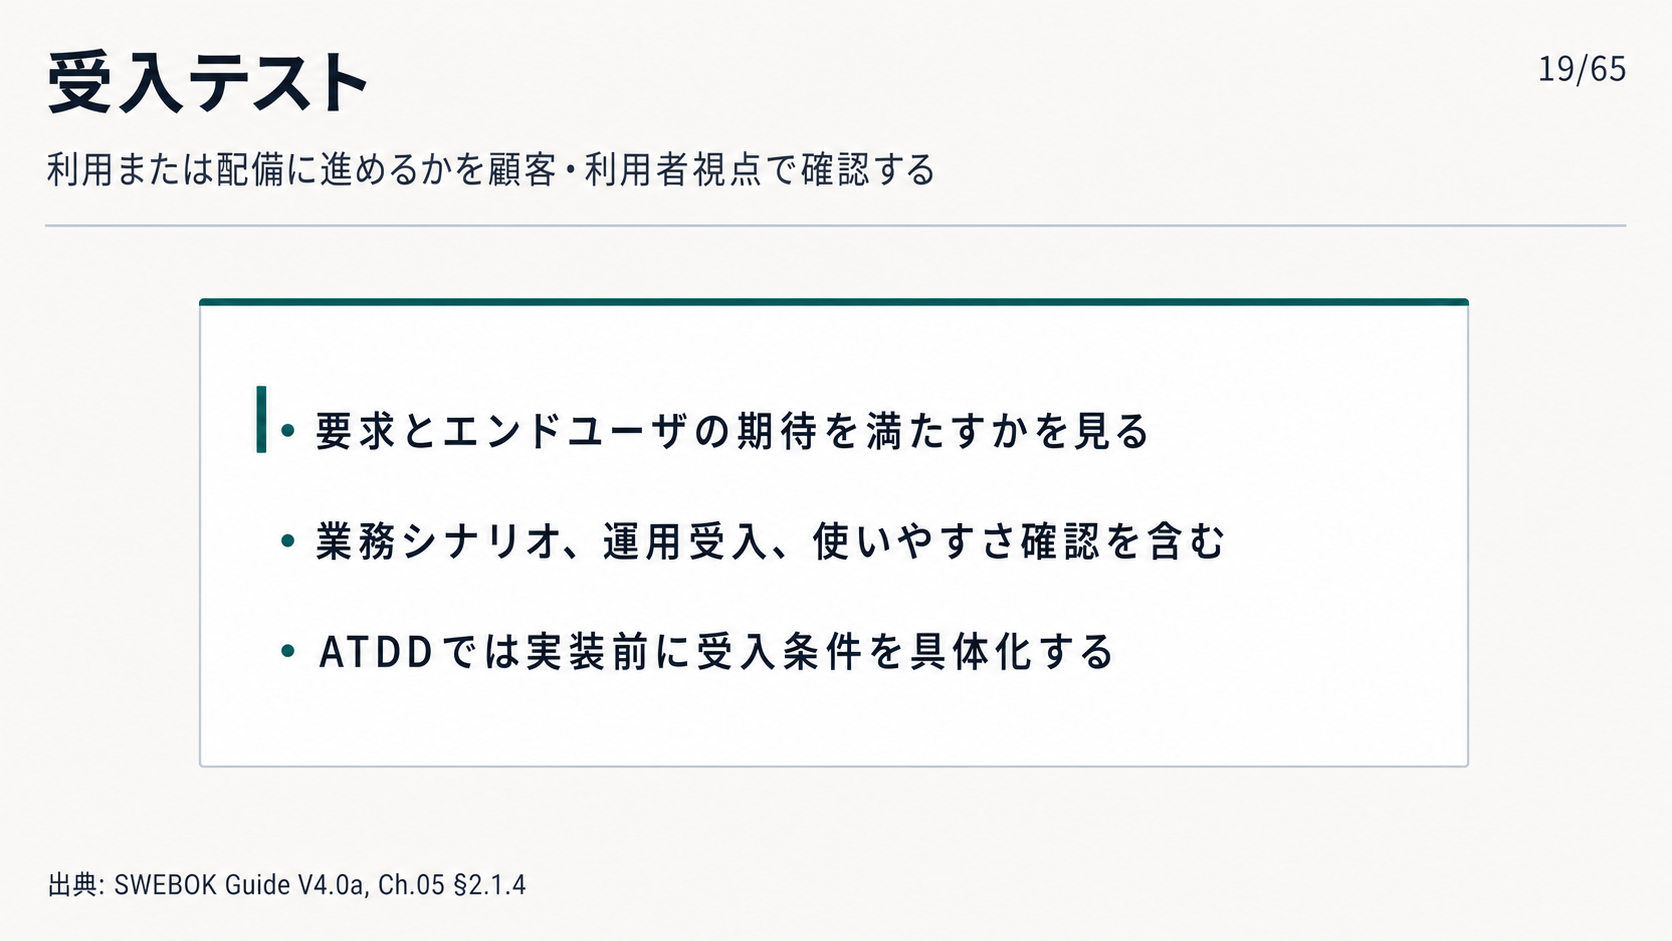
\includegraphics[width=0.96\linewidth]{assets/generated_figures/ch04/fig-ch04-12.png}}{\fbox{\parbox[c][48mm][c]{0.9\linewidth}{\centering 画像生成待ち\\分散・クラウド構築の概念図}}}
\par\smallskip
\refstepcounter{figure}\label{fig:ch04-12}図 \thefigure: 分散・クラウド構築の概念図
\end{center}
図 \thefigure は、分散・クラウド構築の概念図を視覚的に整理したものである。
\par\smallskip

\subsubsection{異種システムの構築}

異種システムとは、種類の異なる計算単位が組み合わさったシステムである。GPU、デジタル信号処理プロセッサ、マイクロコントローラ、周辺プロセッサなどが含まれる。組込みシステムは、異種システムであることが多い。

異種システムでは、ハードウェアとソフトウェアを同時に設計する必要がある。これをハードウェア/ソフトウェア協調設計という。複数の仕様言語、複数のシミュレーション環境、インタフェースの整合、共同検証が課題になる。FPGA や ASIC を使ったハードウェア側の試作・実装と、ソフトウェア側の低水準言語への変換が並行して進むことがある。

\subsubsection{性能分析とチューニング}

性能は、アーキテクチャ、詳細設計、データ構造、アルゴリズム、コードの書き方に影響される。性能分析は、プログラムの実行時情報を集め、時間がかかっている箇所、頻繁に実行される箇所、資源を多く使う箇所を見つける活動である。

コードチューニングは、コードレベルで性能を改善することである。論理式、ループ、データ変換、関数呼び出し、メモリアクセスなどを見直す。重要なのは、推測ではなく測定に基づいて行うことである。測定せずに最適化すると、本当に遅い場所ではない箇所を複雑にしてしまう危険がある。

\begin{keybox}{性能改善の原則}
まず測定し、ボトルネックを特定し、小さく変更し、再測定する。性能のために可読性を大きく下げる場合は、その理由と測定結果を残す必要がある。
\end{keybox}

\par\smallskip
\begin{center}
\centering
\IfFileExists{assets/generated_figures/ch04/fig-ch04-13.png}{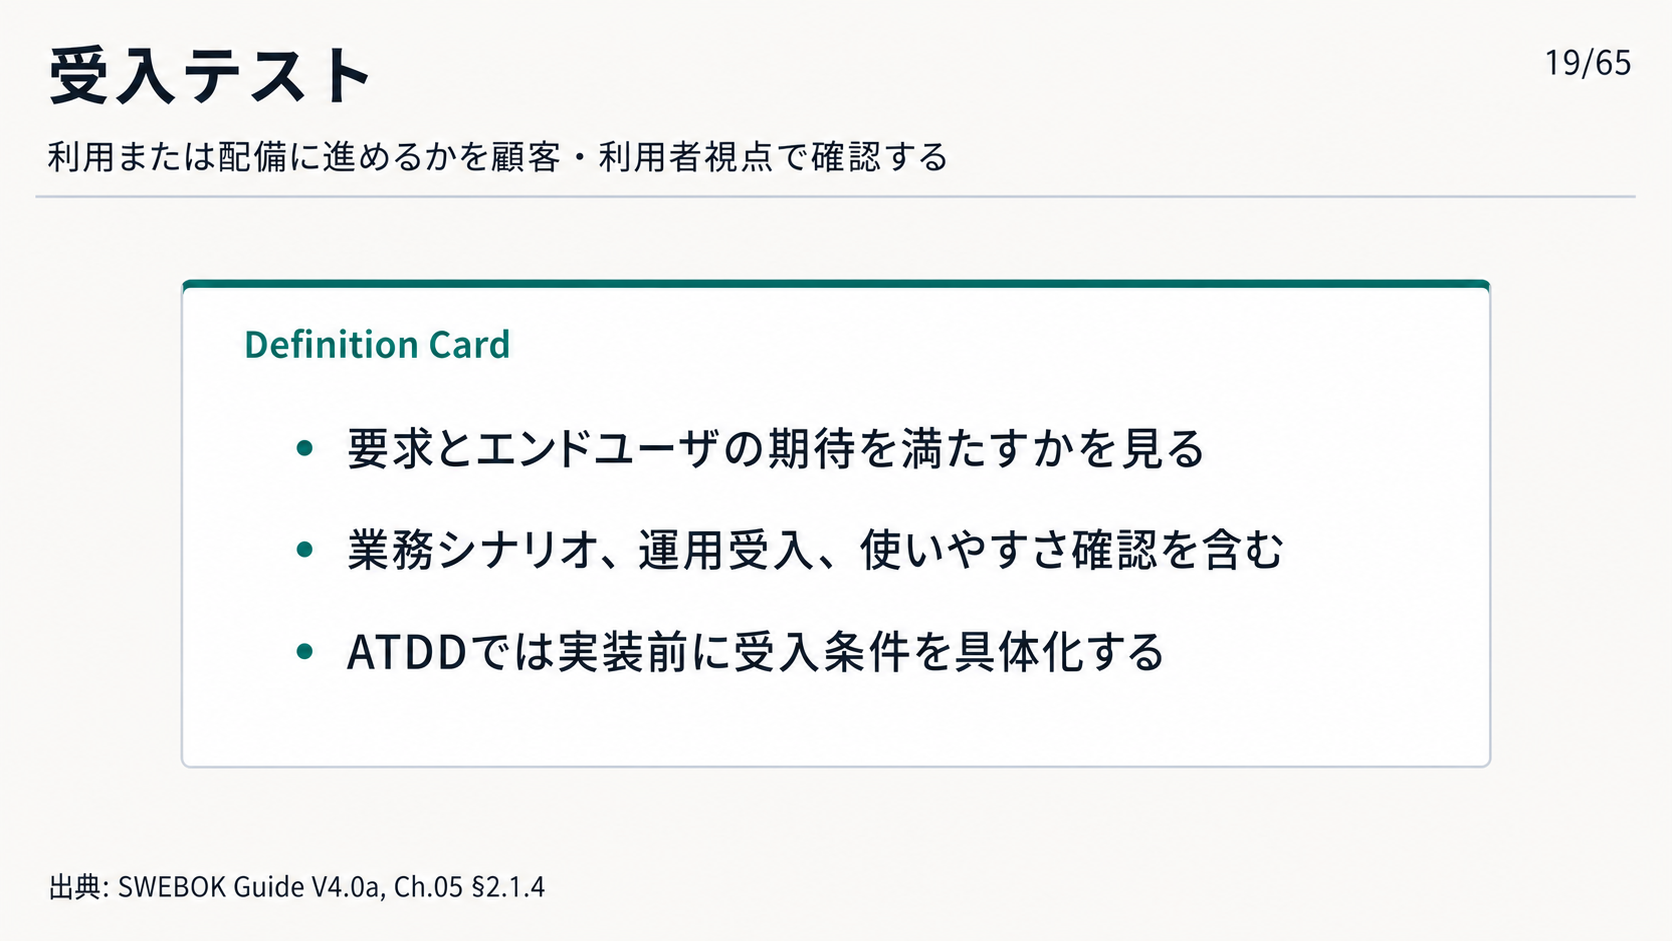
\includegraphics[width=0.96\linewidth]{assets/generated_figures/ch04/fig-ch04-13.png}}{\fbox{\parbox[c][48mm][c]{0.9\linewidth}{\centering 画像生成待ち\\性能分析とチューニングの流れ}}}
\par\smallskip
\refstepcounter{figure}\label{fig:ch04-13}図 \thefigure: 性能分析とチューニングの流れ
\end{center}
図 \thefigure は、性能分析とチューニングの流れを視覚的に整理したものである。
\par\smallskip

\subsubsection{プラットフォーム標準}

プラットフォーム標準は、互換性のある環境でアプリケーションを変更なしに実行しやすくするための標準である。標準サービスや API を定めることで、開発者は特定環境に過度に依存しないアプリケーションを作りやすくなる。

代表例には、エンタープライズ向けの Jakarta Enterprise Edition、Unix 系オペレーティングシステムのインタフェース標準である POSIX、Web アプリケーションの標準を支える HTML5 がある。

標準に従うことは、移植性、相互運用性、保守性を高める。一方で、標準だけでは解決できないプラットフォーム固有の差もあるため、現実の環境での検証が必要である。

\subsubsection{テストファーストプログラミング}

テストファーストプログラミングは、コードを書く前にテストケースを書く開発スタイルである。現在のコードベースでそのテストは失敗する。その後、テストが通るようにコードを書く。テストが通ったら、必要に応じてリファクタリングし、設計を整える。

この方法は、テスト駆動開発としても知られる。テストを先に書くことで、プログラマは要求と設計を先に考える。これにより、要求や設計の問題が早く表面化する。欠陥も早く発見され、修正しやすい。

\par\smallskip
\begin{center}
\centering
\IfFileExists{assets/generated_figures/ch04/fig-ch04-14.png}{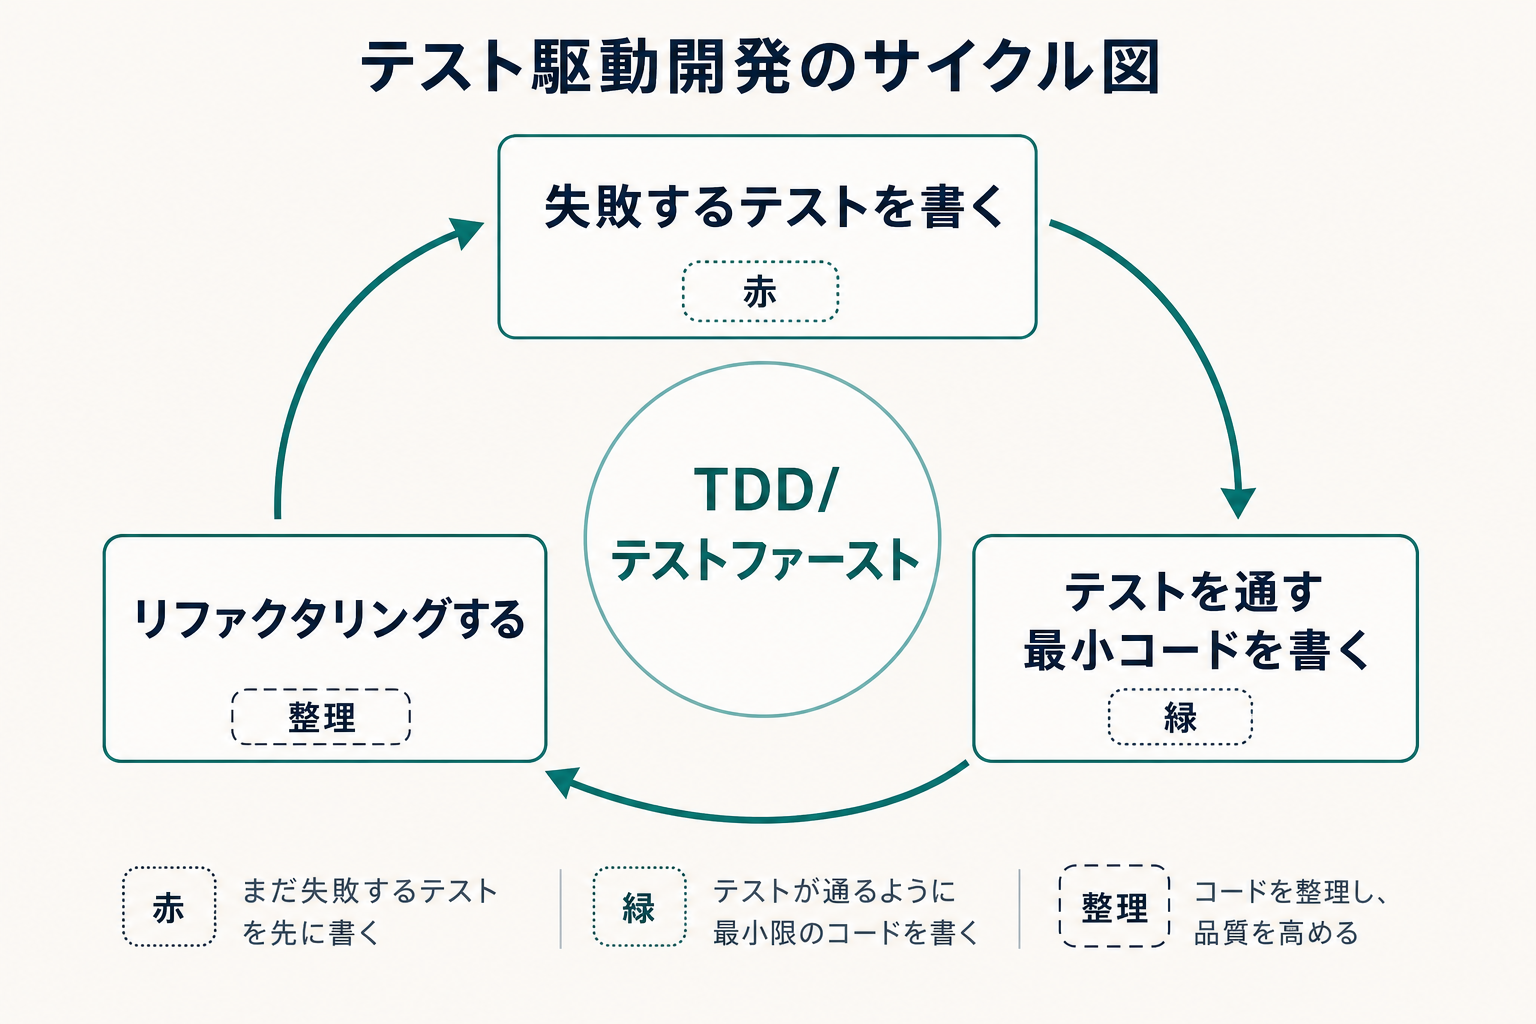
\includegraphics[width=0.96\linewidth]{assets/generated_figures/ch04/fig-ch04-14.png}}{\fbox{\parbox[c][48mm][c]{0.9\linewidth}{\centering 画像生成待ち\\テスト駆動開発のサイクル図}}}
\par\smallskip
\refstepcounter{figure}\label{fig:ch04-14}図 \thefigure: テスト駆動開発のサイクル図
\end{center}
図 \thefigure は、テスト駆動開発のサイクル図を視覚的に整理したものである。
\par\smallskip

\subsubsection{構築のためのフィードバックループ}

構築で重要なのは、早く継続的なフィードバックを得ることである。アジャイル開発では、短い反復で動くソフトウェアを作り、顧客やチームから反応を得る。DevOps では、運用環境からの情報を開発へ戻すことで、実際の性能、信頼性、利用状況を学ぶ。

フィードバックループを支える技法には、自動ビルド、自動テスト、継続的統合、カナリアリリース、A/B テスト、監視、ログ分析がある。カナリアリリースは、全利用者に公開する前に、一部の利用者や環境へ変更を出して問題を観察する方法である。A/B テストは、複数の方式を比較し、実利用のデータから判断する方法である。
